%%
\bigheading{New Tree}
\authors{Gyula Horváth}{Gyula Horváth}{Gyula Horváth}

Trees are point in the plane. Denote the new tree by $Q$.\\
We distinguish two cases.

\heading{Case 1}
The case when there is no point $U$ with the following property: $U$ is collinear with $A$, $Q$ and $Q$ is between $A$ and $U$.\\
Consider the point $B$ on the right side of the line $\overrightarrow{A,Q}$ which has the smallest angle with $\overrightarrow{A,Q}$. If there are more such points, chose the one which is closet to $A$.\\
Similarly, consider the point $C$ on the let side of the line $\overrightarrow{A,Q}$ which has the smallest angle with $\overrightarrow{A,Q}$. If there are more such points, chose the one which is closet to $A$.\\
If there is no such $B$ or $C$ then there is no solution.\\
It is clear that there is a solution if and only if the pair of points $B$ and $C$ is a solution. That is, the triangle with nodes $A$, $B$ and $C$ strictly contains the point $Q$.

\begin{center}
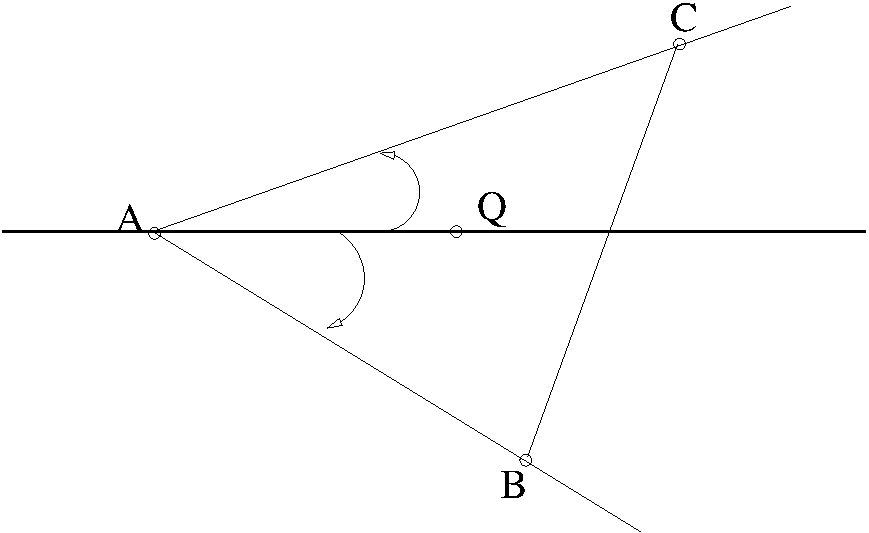
\includegraphics[height=4cm]{img/abra41.pdf}
\end{center}

\heading{Case 2}
There is a point $AA$ with the following property: $AA$ is collinear with $A$, $Q$ and $Q$ is between $A$ and $AA$. If there are several such points, choose the one which is closest to $Q$.\\


In this case a solution exists if and only if there is a point $B$ and there is a point $C$ such that there is no point inside the triangle with nodes $A$,$B$ and $AA$ and the triangle with nodes $A$,$AA$ and $C$ and the pair $B$ $C$ is a solution.\\
%\pdfkep{abra42}{3}{}
\begin{center}
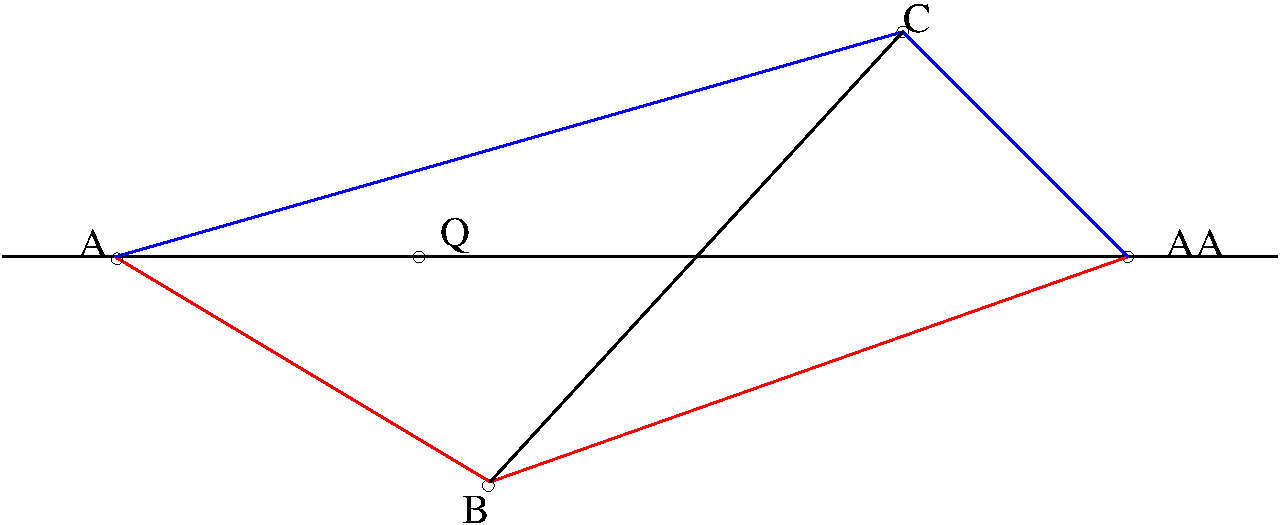
\includegraphics[height=4cm]{img/abra42.pdf}
\end{center}
Indeed, if there is a  point $BB$ in the triangle $A,B,AA$ then replace $B$ with $BB$. Similarly, if there is a point $CC$ in the triangle $A,AA,C$ then replace $C$ with $CC$.\\
%\pdfkep{newtree22}{3}{}
\begin{center}
\centering
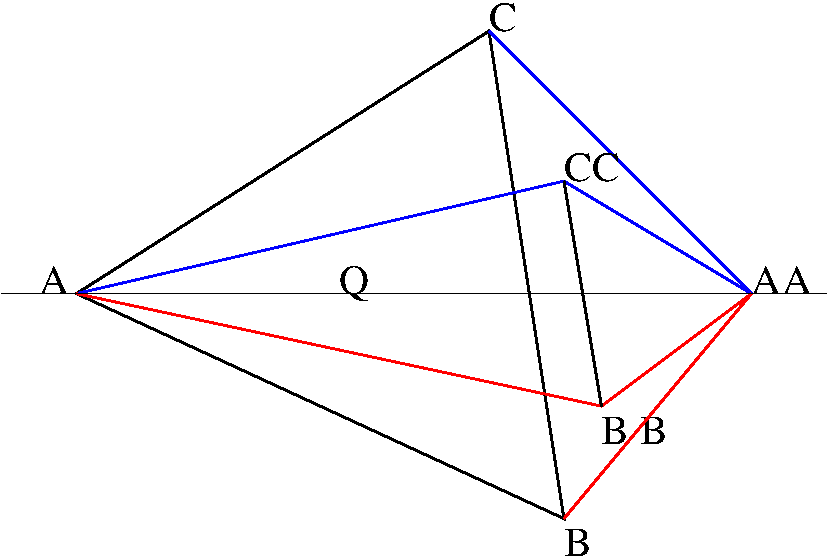
\includegraphics[height=5cm]{img/newtree22.pdf}
\end{center}
%%
Consider the set $R$ of all point $U$ on the right side of the line $\overrightarrow{A,Q}$ with the property that there is no point inside the triangle $\lhd(A,U,AA)$. Sort the set $R$ by the angle at $AA$. Similarly, let $L$ be the set of all point $V$ on the left side of the line $\overrightarrow{A,Q}$ with the property that there is no point inside the triangle $\lhd(A,AA,V)$. Sort the set $L$ by the angle at $A$. \\
We can select solution pair by alternately moving either in $R$ or in $L$ until solution found or exhaust one of the sets.\\
\begin{center}
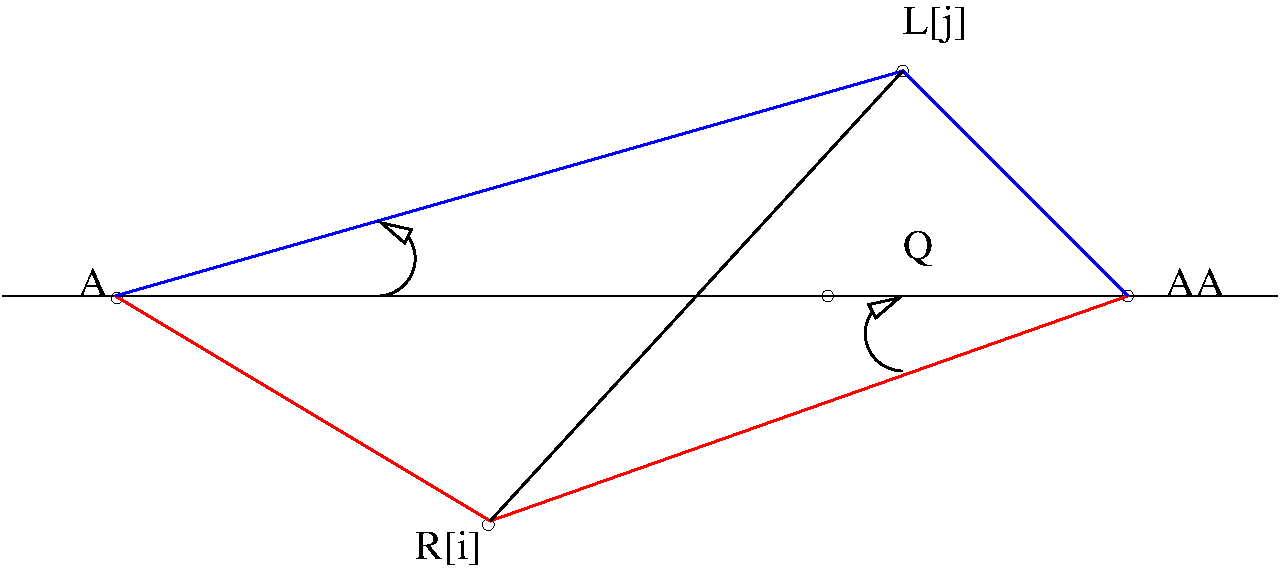
\includegraphics[height=4cm]{img/abra43.pdf}
Move in $R$: $i:=i+1$.\\
\end{center}
\begin{center}
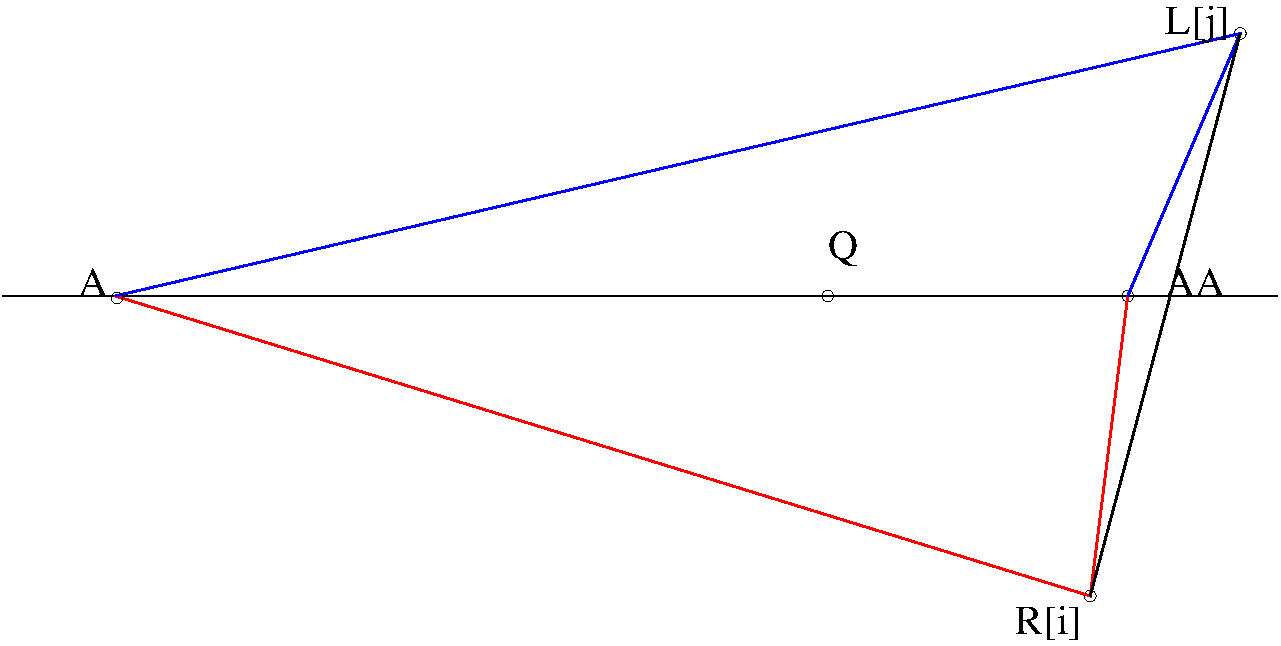
\includegraphics[height=4cm]{img/abra44.pdf}
Move in $L$: $j:=j+1$.\\
\end{center}

The set of points $R$ and $L$ can be constructed by sorting the points by angle.
\\
\emph{\textbf{Running time of the algorithm}}: $O(n \, \log n)$
